\pagenumbering{arabic}
\chapter{Introduction}


\lipsum[12]


Here you can also cite a publication. Like this \cite{Cie2022}.


\section{Thesis structure}

\lipsum[4]


\begin{itemize}
	\item Chapter 1 – \textbf{Introduction}
	
	This chapter contains a the introduction. 
	
	\item Chapter 2 – \textbf{Some nice chapter}
	
	The chapter outlines some great results.
	
	\item Chapter 3 – \textbf{Experimental}
	
	This part of the dissertation describes experimental details.

	\item Chapter 4 - \textbf{Conclusions}
	
	This chapter contains the conclusions.

	\item Appendix - \textbf{Academic achievements}
	
	The publications and conferences at which  the results were presented are listed here. 
\end{itemize}

\section{Motivations}

\lipsum[5-7]


\section{Some section with an equation and citations}


Here the Equation \ref{reaction-oxidation-sto} starts:
\begin{equation}
	k \cdot \ce{ SrTiO3} \ce{->} p \cdot \ce{ SrTiO3}  +   q \cdot \ce{SrO (SrTiO3)_n} +  q \cdot \ce{TiO2},
	\label{reaction-oxidation-sto}
\end{equation}
where $k = q\cdot (n+1) + p$. And here it ends.


\subsection{A subsection}

\lipsum[12]

\section{Some section with a figure} \label{section-with-figure}

\lipsum[15-16]
\begin{figure} [!h]
	\centering
	%\captionsetup{justification=centering}
	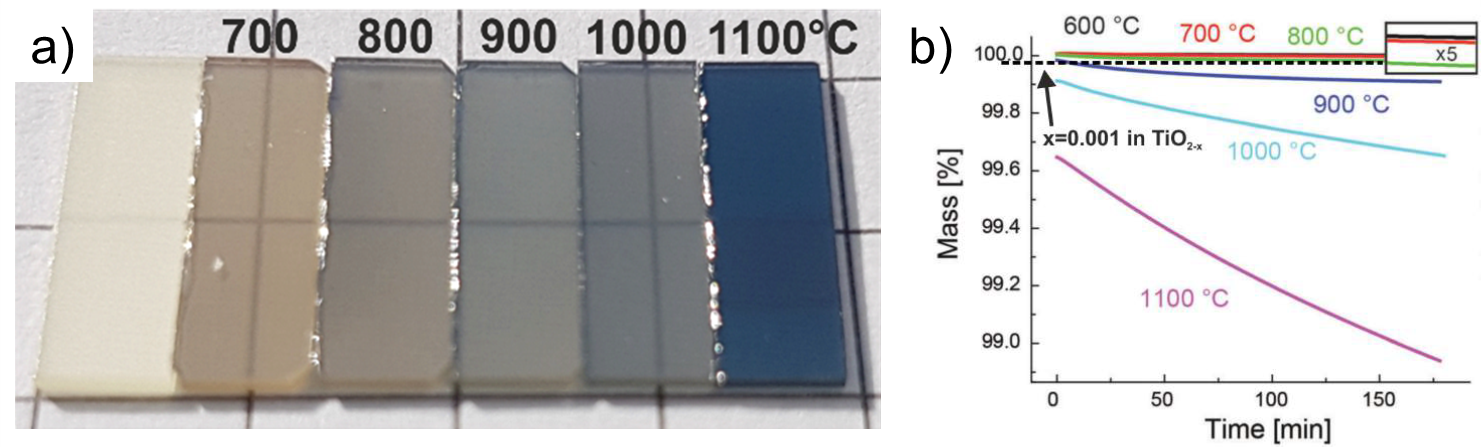
\includegraphics[width=14cm,height=8cm,keepaspectratio]{figures/introduction/annealing-intro}
	\setlength\belowcaptionskip{3pt}
	\caption{Some figure with with part a) and b).}
	\label{some-figure}
\end{figure}


We are in the Section \ref{section-with-figure} with Figure \ref{some-figure}.


\lipsum[19-20]






